\documentclass[10pt]{article}
\usepackage[polish]{babel}
\usepackage[utf8]{inputenc}
\usepackage[T1]{fontenc}
\usepackage{amsmath}
\usepackage{amsfonts}
\usepackage{amssymb}
\usepackage[version=4]{mhchem}
\usepackage{stmaryrd}
\usepackage{graphicx}
\usepackage[export]{adjustbox}
\graphicspath{ {./images/} }

\title{LIGA MATEMATYCZNA im. Zdzisława Matuskiego PAŹDZIERNIK 2019 SZKOŁA PODSTAWOWA klasy VII - VIII }

\author{}
\date{}


\begin{document}
\maketitle
\section*{ZADANIE 1.}
Z sześciu jednakowych trójkątów prostokątnych o kącie ostrym \(60^{\circ}\) i najkrótszym boku 10 cm zbudowano równoległobok \(A B C D\). Oblicz długości obu przekątnych tego równoległoboku.\\
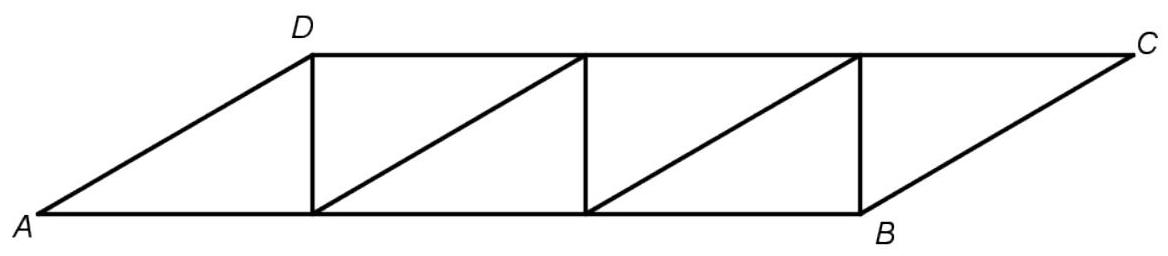
\includegraphics[max width=\textwidth, center]{2024_11_21_1f05046b5731d06af56cg-1}

\section*{ZADANIE 2.}
Adam napisał cztery razy z rzędu liczbę dwucyfrową. Wykaż, że otrzymana liczba ośmiocyfrowa jest podzielna przez 101.

\section*{ZADANIE 3.}
Jedna przekątna pewnego czworokąta dzieli go na dwa trójkąty o obwodach 20 i 40, a druga na trójkąty o obwodach 30 i 50 . Wiedząc, że suma długości przekątnych jest równa 26, oblicz obwód czworokąta.

\section*{ZADANIE 4.}
Rozwiąż układ równań

\[
\left\{\begin{array}{l}
x y=6 \\
y z=12 \\
x z=8 .
\end{array}\right.
\]

\section*{ZADANIE 5.}
Dwa tysiące dziewiętnaście liczb zapisano jedna za drugą. Wiadomo, że suma każdych trzech kolejnych z nich jest równa 200. Pierwsza z nich jest równa 19, a ostatnia 99. Wyznacz pozostałe 2017 liczb.


\end{document}